% Rebuilt from the uploaded HTML/SVG figure as a printable TikZ figure, recolored with the requested muted palette.
% Layout calculation used to avoid cramming:
% A4 landscape width = 29.7 cm. With 1.0 cm left/right print margin, usable width = 27.7 cm.
% Chosen panel width P = 8.2 cm and arrow lane A = 1.1 cm.
% Total figure width = 3P + 2A = 3(8.2) + 2(1.1) = 26.8 cm.
% Remaining horizontal slack = 27.7 - 26.8 = 0.9 cm, i.e. 0.45 cm on each side.
% Chosen panel height = 6.6 cm. Two rows plus vertical gap = 2(6.6) + 0.9 = 14.1 cm.
% A4 landscape height = 21.0 cm, leaving about 6.9 cm vertical slack for clean printing.
\documentclass[a4paper,landscape]{article}
\usepackage[margin=1cm]{geometry}
\usepackage{tikz}
\usepackage{amsmath,amssymb}
\usetikzlibrary{arrows.meta,calc,positioning,patterns}
\pagestyle{empty}
\setlength{\parindent}{0pt}


\definecolor{ink}{HTML}{111827}          % text only: kept dark for print readability
\definecolor{mutedText}{HTML}{374151}    % secondary text only

% User muted palette for visual elements
\definecolor{mistyblue}{HTML}{A3BFD9}
\definecolor{slateblue}{HTML}{7A90B2}
\definecolor{sagegreen}{HTML}{A3BFA3}
\definecolor{dustyteal}{HTML}{6E8B8B}
\definecolor{softgray}{HTML}{D8D8D8}
\definecolor{deepmutedblue}{HTML}{4A5A6A}

% Semantic aliases: all visible diagram colors below are derived from the palette above.
\colorlet{lineGrey}{softgray}
\colorlet{cellFill}{softgray!55}
\colorlet{softBlue}{mistyblue!28}
\colorlet{softSand}{sagegreen!24}
\colorlet{selectBlue}{slateblue!72}
\colorlet{selectBlueDark}{deepmutedblue}
\colorlet{pruneRed}{deepmutedblue}
\colorlet{pruneRedDark}{deepmutedblue}
\colorlet{keepTeal}{sagegreen!82}
\colorlet{keepTealDark}{dustyteal}
\colorlet{hessGold}{mistyblue!78}
\colorlet{hessGoldDark}{slateblue}
\colorlet{violetSoft}{mistyblue!18}


\tikzset{
  panel/.style={rounded corners=3.5pt, draw=lineGrey, line width=0.65pt, fill=white},
  headerTop/.style={rounded corners=3.5pt, draw=none, fill=softBlue},
  headerBot/.style={rounded corners=3.5pt, draw=none, fill=softSand},
  title/.style={font=\bfseries\large, text=ink, align=center},
  smallnote/.style={font=\small, text=mutedText, align=center},
  formula/.style={font=\small, text=ink, align=center},
  arrow/.style={-{Stealth[length=3.5mm,width=2.7mm]}, line width=0.9pt, draw=deepmutedblue},
  cell/.style={rounded corners=1.2pt, draw=lineGrey, line width=0.35pt, fill=cellFill},
  chosen/.style={rounded corners=1.2pt, draw=selectBlueDark, line width=0.65pt, fill=selectBlue!75},
  pruned/.style={rounded corners=1.2pt, draw=pruneRed, line width=0.95pt, fill=white},
  kept/.style={rounded corners=1.2pt, draw=keepTealDark, line width=0.65pt, fill=keepTeal!65},
  hcell/.style={rounded corners=1.2pt, draw=hessGoldDark, line width=0.55pt, fill=hessGold!50}
}

\newcommand{\PanelW}{8.2}
\newcommand{\PanelH}{6.6}
\newcommand{\Gap}{1.1}

\begin{document}
\vspace*{1.1cm}
\begin{center}
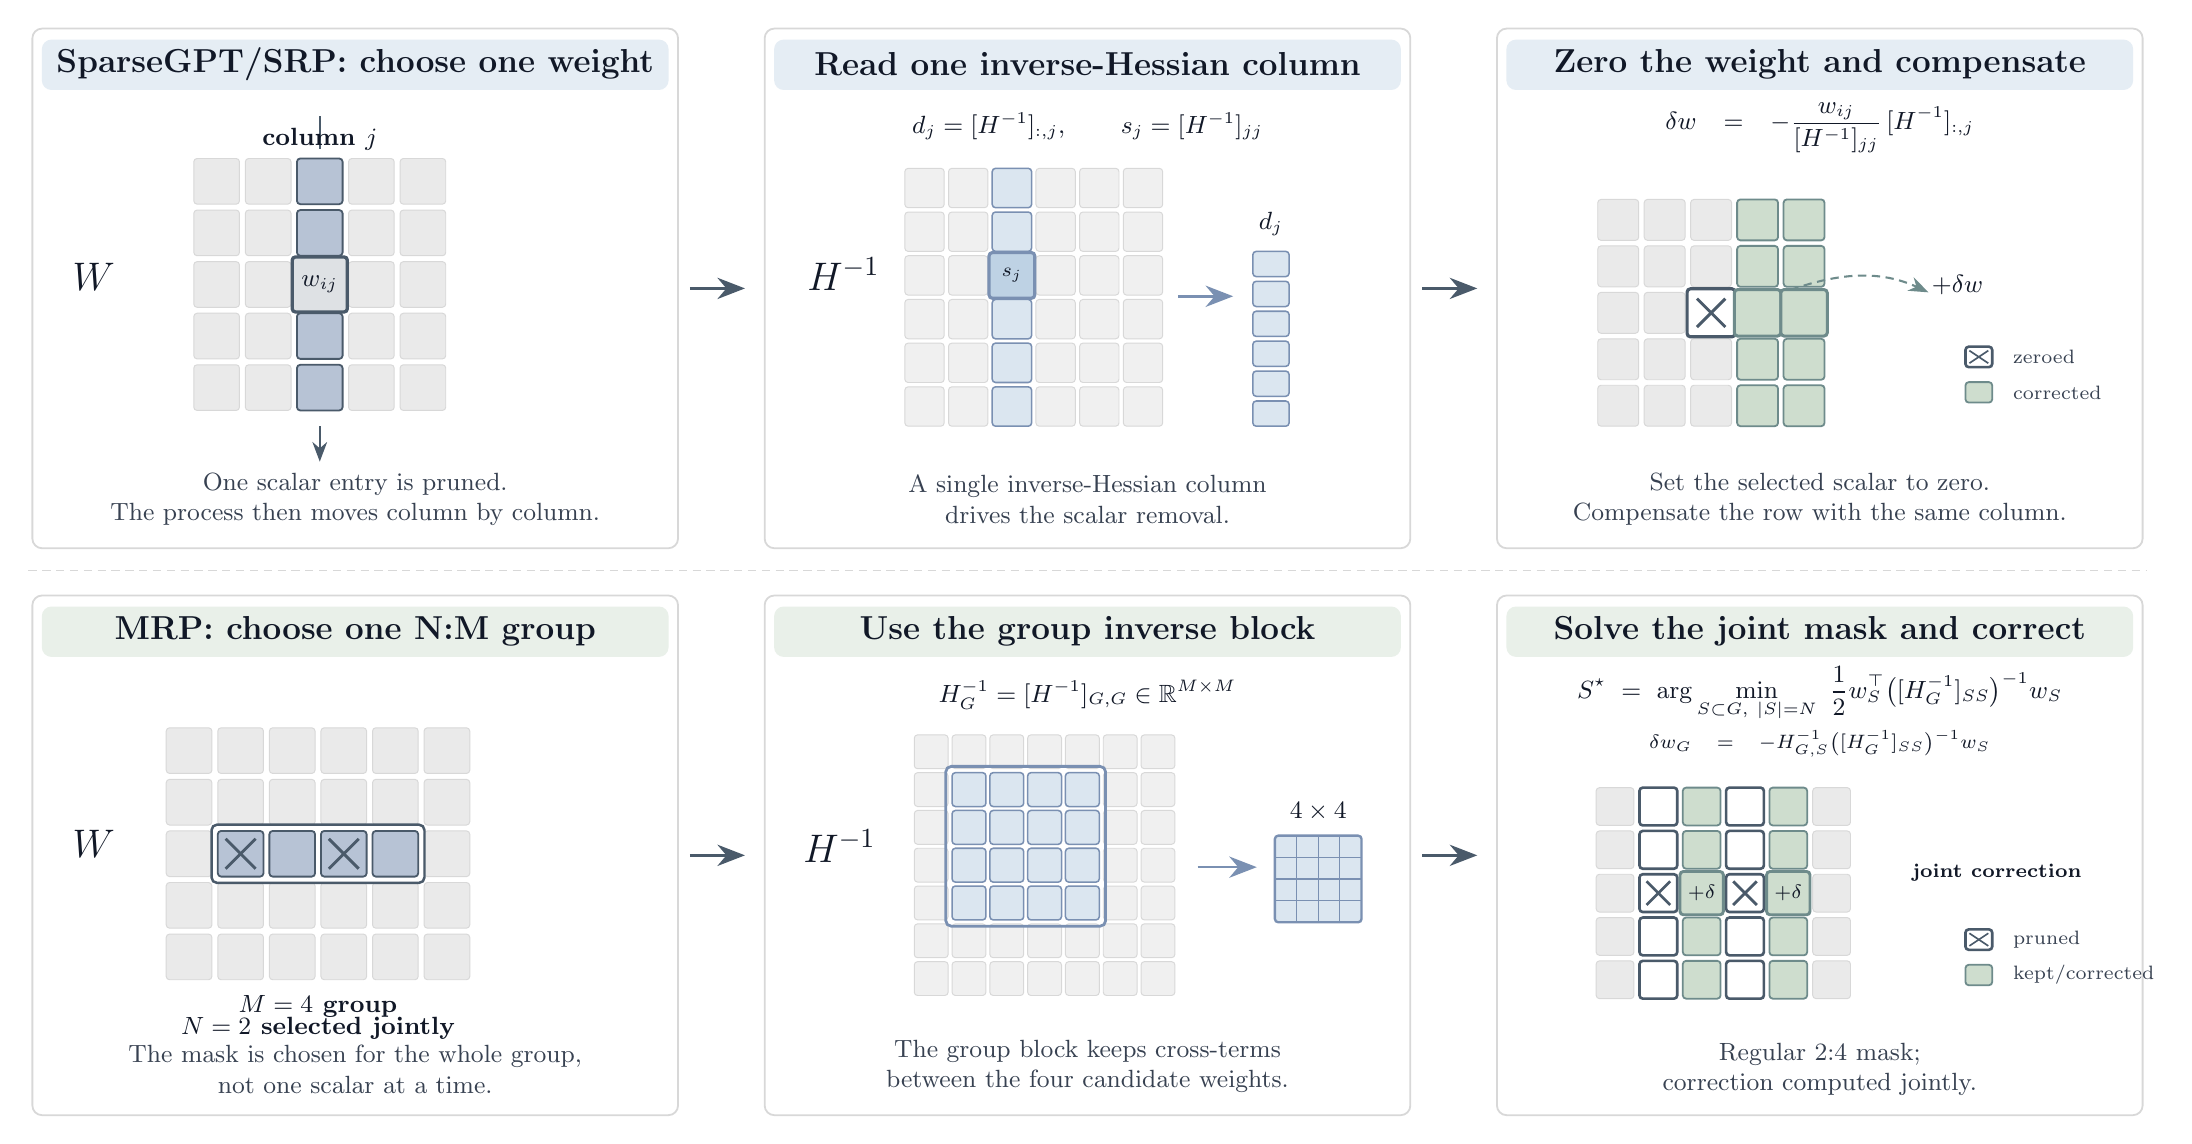
\begin{tikzpicture}[x=1cm,y=1cm]

% Row and column anchors
\coordinate (T0) at (0,7.2);
\coordinate (T1) at (9.3,7.2);
\coordinate (T2) at (18.6,7.2);
\coordinate (B0) at (0,0);
\coordinate (B1) at (9.3,0);
\coordinate (B2) at (18.6,0);

% ----- helper: panel frames -----
\foreach \P/\Hdr/\Name in {T0/headerTop/{SparseGPT/SRP: choose one weight},T1/headerTop/{Read one inverse-Hessian column},T2/headerTop/{Zero the weight and compensate},B0/headerBot/{MRP: choose one N:M group},B1/headerBot/{Use the group inverse block},B2/headerBot/{Solve the joint mask and correct}}{
  \begin{scope}[shift={(\P)}]
    \draw[panel] (0,0) rectangle (\PanelW,\PanelH);
    \path[\Hdr] (0.12,5.82) rectangle (8.08,6.46);
    \node[title,text width=7.7cm] at (4.1,6.15) {\Name};
  \end{scope}
}

% row divider, no boxed label
\draw[densely dashed, lineGrey, line width=0.55pt] (-0.05,6.92) -- (26.85,6.92);

% arrows
\draw[arrow] (8.35,10.50) -- (9.05,10.50);
\draw[arrow] (17.65,10.50) -- (18.35,10.50);
\draw[arrow] (8.35,3.30) -- (9.05,3.30);
\draw[arrow] (17.65,3.30) -- (18.35,3.30);

% ===================== TOP PANEL 1 =====================
\begin{scope}[shift={(T0)}]
  \node[font=\Large\itshape, text=ink] at (0.78,3.45) {$W$};
  \def\s{0.58}
  \def\g{0.075}
  \def\x0{2.05}
  \def\y0{1.75}
  % matrix cells, row 0 at top
  \foreach \r in {0,...,4}{
    \foreach \c in {0,...,4}{
      \pgfmathsetmacro{\x}{\x0+\c*(\s+\g)}
      \pgfmathsetmacro{\y}{\y0+(4-\r)*(\s+\g)}
      \ifnum\c=2
        \draw[chosen] (\x,\y) rectangle +(\s,\s);
      \else
        \draw[cell] (\x,\y) rectangle +(\s,\s);
      \fi
    }
  }
  % selected weight
  \pgfmathsetmacro{\tx}{\x0+2*(\s+\g)}
  \pgfmathsetmacro{\ty}{\y0+2*(\s+\g)}
  \draw[pruned, line width=1.2pt, fill=pruneRed!18] ({\tx-0.06},{\ty-0.06}) rectangle +({\s+0.12},{\s+0.12});
  \node[font=\bfseries\small, text=ink] at ({\tx+0.5*\s},{\ty+0.5*\s}) {$w_{ij}$};
  \draw[pruneRed, line width=0.6pt] ({\tx+0.5*\s},{\y0+5*(\s+\g)+0.05}) -- ++(0,0.42);
  \node[font=\small\bfseries, text=ink] at ({\tx+0.5*\s},5.20) {column $j$};
  \draw[pruneRed, -{Stealth[length=2.5mm]}, line width=0.65pt] ({\tx+0.5*\s},1.55) -- ++(0,-0.45);
  \node[smallnote,text width=6.9cm] at (4.1,0.62) {One scalar entry is pruned.\\The process then moves column by column.};
\end{scope}

% ===================== TOP PANEL 2 =====================
\begin{scope}[shift={(T1)}]
  \node[formula] at (4.1,5.36) {$d_j = [H^{-1}]_{:,j},\qquad s_j=[H^{-1}]_{jj}$};
  \node[font=\Large\itshape, text=ink] at (1.00,3.48) {$H^{-1}$};
  \def\s{0.50}
  \def\g{0.055}
  \def\x0{1.78}
  \def\y0{1.55}
  \foreach \r in {0,...,5}{
    \foreach \c in {0,...,5}{
      \pgfmathsetmacro{\x}{\x0+\c*(\s+\g)}
      \pgfmathsetmacro{\y}{\y0+(5-\r)*(\s+\g)}
      \ifnum\c=2
        \draw[hcell] (\x,\y) rectangle +(\s,\s);
      \else
        \draw[cell, fill=cellFill!70] (\x,\y) rectangle +(\s,\s);
      \fi
    }
  }
  % diagonal scalar [H^-1]jj emphasized
  \pgfmathsetmacro{\dx}{\x0+2*(\s+\g)}
  \pgfmathsetmacro{\dy}{\y0+(5-2)*(\s+\g)}
  \draw[hcell, line width=1.15pt, fill=hessGold!90] ({\dx-0.04},{\dy-0.04}) rectangle +({\s+0.08},{\s+0.08});
  \node[font=\scriptsize\bfseries, text=ink] at ({\dx+0.5*\s},{\dy+0.5*\s}) {$s_j$};
  % vector extraction
  \draw[arrow, draw=hessGoldDark] (5.25,3.20) -- (5.95,3.20);
  \foreach \r in {0,...,5}{
    \pgfmathsetmacro{\y}{1.55+(5-\r)*(0.38)}
    \draw[hcell] (6.20,\y) rectangle +(0.46,0.32);
  }
  \node[font=\small\bfseries, text=ink] at (6.43,4.12) {$d_j$};
  \node[smallnote,text width=6.9cm] at (4.1,0.62) {A single inverse-Hessian column\\drives the scalar removal.};
\end{scope}

% ===================== TOP PANEL 3 =====================
\begin{scope}[shift={(T2)}]
  \node[formula,text width=7.55cm] at (4.1,5.34)
    {$\displaystyle \delta w = -\frac{w_{ij}}{[H^{-1}]_{jj}}\,[H^{-1}]_{:,j}$};
  \def\s{0.52}
  \def\g{0.070}
  \def\x0{1.28}
  \def\y0{1.55}
  \foreach \r in {0,...,4}{
    \foreach \c in {0,...,4}{
      \pgfmathsetmacro{\x}{\x0+\c*(\s+\g)}
      \pgfmathsetmacro{\y}{\y0+(4-\r)*(\s+\g)}
      \ifnum\c=3
        \draw[kept] (\x,\y) rectangle +(\s,\s);
      \else\ifnum\c=4
        \draw[kept] (\x,\y) rectangle +(\s,\s);
      \else
        \draw[cell] (\x,\y) rectangle +(\s,\s);
      \fi\fi
    }
  }
  \pgfmathsetmacro{\px}{\x0+2*(\s+\g)}
  \pgfmathsetmacro{\py}{\y0+2*(\s+\g)}
  \draw[pruned, line width=1.15pt] ({\px-0.045},{\py-0.045}) rectangle +({\s+0.09},{\s+0.09});
  \draw[pruneRed, line width=1.05pt] ({\px+0.08},{\py+0.08}) -- ({\px+\s-0.08},{\py+\s-0.08});
  \draw[pruneRed, line width=1.05pt] ({\px+\s-0.08},{\py+0.08}) -- ({\px+0.08},{\py+\s-0.08});
  \node[font=\bfseries\small, text=ink] at (5.85,3.34) {$+\delta w$};
  \draw[-{Stealth[length=2.5mm]}, draw=keepTealDark, line width=0.75pt, densely dashed]
    ({\px+\s+0.10},{\py+0.28}) .. controls +(0.95,0.45) and +(-0.75,0.35) .. (5.48,3.25);
  \draw[kept, line width=1.1pt] ({\x0+3*(\s+\g)-0.035},{\py-0.035}) rectangle +({\s+0.07},{\s+0.07});
  \draw[kept, line width=1.1pt] ({\x0+4*(\s+\g)-0.035},{\py-0.035}) rectangle +({\s+0.07},{\s+0.07});
  \begin{scope}[shift={(5.95,1.75)}]
    \draw[pruned] (0,0.55) rectangle +(0.34,0.26);
    \draw[pruneRed,line width=0.6pt] (0.05,0.60)--(0.29,0.76);
    \draw[pruneRed,line width=0.6pt] (0.29,0.60)--(0.05,0.76);
    \node[anchor=west,font=\scriptsize,text=mutedText] at (0.48,0.68) {zeroed};
    \draw[kept] (0,0.10) rectangle +(0.34,0.26);
    \node[anchor=west,font=\scriptsize,text=mutedText] at (0.48,0.23) {corrected};
  \end{scope}
  \node[smallnote,text width=7.1cm] at (4.1,0.62) {Set the selected scalar to zero.\\Compensate the row with the same column.};
\end{scope}

% ===================== BOTTOM PANEL 1 =====================
\begin{scope}[shift={(B0)}]
  \node[font=\Large\itshape, text=ink] at (0.78,3.45) {$W$};
  \def\s{0.58}
  \def\g{0.075}
  \def\x0{1.70}
  \def\y0{1.72}
  \foreach \r in {0,...,4}{
    \foreach \c in {0,...,5}{
      \pgfmathsetmacro{\x}{\x0+\c*(\s+\g)}
      \pgfmathsetmacro{\y}{\y0+(4-\r)*(\s+\g)}
      \ifnum\r=2
        \ifnum\c>0
          \ifnum\c<5
            \draw[chosen] (\x,\y) rectangle +(\s,\s);
          \else
            \draw[cell] (\x,\y) rectangle +(\s,\s);
          \fi
        \else
          \draw[cell] (\x,\y) rectangle +(\s,\s);
        \fi
      \else
        \draw[cell] (\x,\y) rectangle +(\s,\s);
      \fi
    }
  }
  % group brace and pruned candidates inside M=4 group
  \pgfmathsetmacro{\gx}{\x0+1*(\s+\g)}
  \pgfmathsetmacro{\gy}{\y0+2*(\s+\g)}
  \draw[selectBlueDark, line width=0.9pt, rounded corners=2pt] ({\gx-0.08},{\gy-0.08}) rectangle ({\gx+4*\s+3*\g+0.08},{\gy+\s+0.08});
  \foreach \c in {1,3}{
    \pgfmathsetmacro{\xx}{\x0+\c*(\s+\g)}
    \draw[pruneRedDark,line width=1.05pt] ({\xx+0.10},{\gy+0.10}) -- ({\xx+\s-0.10},{\gy+\s-0.10});
    \draw[pruneRedDark,line width=1.05pt] ({\xx+\s-0.10},{\gy+0.10}) -- ({\xx+0.10},{\gy+\s-0.10});
  }
  \node[font=\small\bfseries,text=ink] at ({\gx+2*\s+1.5*\g},1.38) {$M=4$ group};
  \node[font=\small\bfseries,text=ink] at ({\gx+2*\s+1.5*\g},1.10) {$N=2$ selected jointly};
  \node[smallnote,text width=7.1cm] at (4.1,0.58) {The mask is chosen for the whole group,\\not one scalar at a time.};
\end{scope}

% ===================== BOTTOM PANEL 2 =====================
\begin{scope}[shift={(B1)}]
  \node[formula] at (4.1,5.34) {$H_G^{-1} = [H^{-1}]_{G,G}\in\mathbb{R}^{M\times M}$};
  \node[font=\Large\itshape, text=ink] at (0.95,3.42) {$H^{-1}$};
  \def\s{0.43}
  \def\g{0.050}
  \def\x0{1.90}
  \def\y0{1.52}
  \foreach \r in {0,...,6}{
    \foreach \c in {0,...,6}{
      \pgfmathsetmacro{\x}{\x0+\c*(\s+\g)}
      \pgfmathsetmacro{\y}{\y0+(6-\r)*(\s+\g)}
      \ifnum\r>0
        \ifnum\r<5
          \ifnum\c>0
            \ifnum\c<5
              \draw[hcell] (\x,\y) rectangle +(\s,\s);
            \else
              \draw[cell, fill=cellFill!70] (\x,\y) rectangle +(\s,\s);
            \fi
          \else
            \draw[cell, fill=cellFill!70] (\x,\y) rectangle +(\s,\s);
          \fi
        \else
          \draw[cell, fill=cellFill!70] (\x,\y) rectangle +(\s,\s);
        \fi
      \else
        \draw[cell, fill=cellFill!70] (\x,\y) rectangle +(\s,\s);
      \fi
    }
  }
  \pgfmathsetmacro{\bx}{\x0+1*(\s+\g)}
  \pgfmathsetmacro{\by}{\y0+2*(\s+\g)}
  \draw[hessGoldDark, line width=1.0pt, rounded corners=2pt] ({\bx-0.08},{\by-0.08}) rectangle ({\bx+4*\s+3*\g+0.08},{\by+4*\s+3*\g+0.08});
  \draw[arrow, draw=hessGoldDark] (5.50,3.15) -- (6.25,3.15);
  \draw[hcell, line width=0.85pt] (6.48,2.45) rectangle +(1.10,1.10);
  \draw[hessGoldDark, line width=0.45pt] (6.755,2.45)--++(0,1.10);
  \draw[hessGoldDark, line width=0.45pt] (7.03,2.45)--++(0,1.10);
  \draw[hessGoldDark, line width=0.45pt] (7.305,2.45)--++(0,1.10);
  \draw[hessGoldDark, line width=0.45pt] (6.48,2.725)--++(1.10,0);
  \draw[hessGoldDark, line width=0.45pt] (6.48,3.00)--++(1.10,0);
  \draw[hessGoldDark, line width=0.45pt] (6.48,3.275)--++(1.10,0);
  \node[font=\small\bfseries,text=ink] at (7.03,3.85) {$4\times4$};
  \node[smallnote,text width=7.2cm] at (4.1,0.62) {The group block keeps cross-terms\\between the four candidate weights.};
\end{scope}

% ===================== BOTTOM PANEL 3 =====================
\begin{scope}[shift={(B2)}]
  \node[formula,text width=7.65cm] at (4.1,5.35)
    {$\displaystyle S^\star=\arg\min_{S\subset G,\ |S|=N}\ \frac12 w_S^\top\big([H_G^{-1}]_{SS}\big)^{-1}w_S$};
  \def\s{0.48}
  \def\g{0.070}
  \def\x0{1.26}
  \def\y0{1.48}
  \foreach \r in {0,...,4}{
    \foreach \c in {0,...,5}{
      \pgfmathsetmacro{\x}{\x0+\c*(\s+\g)}
      \pgfmathsetmacro{\y}{\y0+(4-\r)*(\s+\g)}
      \ifnum\c=1
        \draw[pruned] (\x,\y) rectangle +(\s,\s);
      \else\ifnum\c=3
        \draw[pruned] (\x,\y) rectangle +(\s,\s);
      \else\ifnum\c=2
        \draw[kept] (\x,\y) rectangle +(\s,\s);
      \else\ifnum\c=4
        \draw[kept] (\x,\y) rectangle +(\s,\s);
      \else
        \draw[cell] (\x,\y) rectangle +(\s,\s);
      \fi\fi\fi\fi
    }
  }
  % emphasize target row and symbols
  \pgfmathsetmacro{\ry}{\y0+2*(\s+\g)}
  \foreach \c in {1,3}{
    \pgfmathsetmacro{\xx}{\x0+\c*(\s+\g)}
    \draw[pruneRedDark,line width=1.0pt] ({\xx+0.09},{\ry+0.09}) -- ({\xx+\s-0.09},{\ry+\s-0.09});
    \draw[pruneRedDark,line width=1.0pt] ({\xx+\s-0.09},{\ry+0.09}) -- ({\xx+0.09},{\ry+\s-0.09});
  }
  \foreach \c in {2,4}{
    \pgfmathsetmacro{\xx}{\x0+\c*(\s+\g)}
    \draw[kept,line width=1.05pt] ({\xx-0.035},{\ry-0.035}) rectangle +({\s+0.07},{\s+0.07});
    \node[font=\scriptsize\bfseries,text=ink] at ({\xx+0.5*\s},{\ry+0.5*\s}) {$+\delta$};
  }
  \node[formula,text width=7.65cm, font=\scriptsize] at (4.1,4.72)
    {$\displaystyle \delta w_G=-H_{G,S}^{-1}\big([H_G^{-1}]_{SS}\big)^{-1}w_S$};
  \node[font=\scriptsize\bfseries,text=ink] at (6.35,3.08) {joint correction};
  \begin{scope}[shift={(5.95,1.55)}]
    \draw[pruned] (0,0.55) rectangle +(0.34,0.26);
    \draw[pruneRedDark,line width=0.6pt] (0.05,0.60)--(0.29,0.76);
    \draw[pruneRedDark,line width=0.6pt] (0.29,0.60)--(0.05,0.76);
    \node[anchor=west,font=\scriptsize,text=mutedText] at (0.48,0.68) {pruned};
    \draw[kept] (0,0.10) rectangle +(0.34,0.26);
    \node[anchor=west,font=\scriptsize,text=mutedText] at (0.48,0.23) {kept/corrected};
  \end{scope}
  \node[smallnote,text width=7.2cm] at (4.1,0.58) {Regular 2:4 mask;\\correction computed jointly.};
\end{scope}

\end{tikzpicture}
\end{center}
\end{document}
